\documentclass{article}
\usepackage{graphicx} % Required for inserting images
\usepackage{listings}
\usepackage{amsmath}

\title{Task 5}
\author{} 
\date{}

\begin{document}

\maketitle

\section*{5.1) : Answer}

The player needs to choose the right-hand lift as a = 0, boolean False.
\\On the left hand of the equivalence we have inside the bracket the proposition\[p
 \oplus q
\] as p and q are false the bracket is equal to false. 

\vspace{0.3cm} The proposition 
\[
(p \oplus q) \oplus r
\] as both the bracket and r are false the proposition is false, therefore the left-hand side is equal to false.
 As the variable a is a constant and does not affect the logical result, we resolve the equivalent proposition first and multiply a by the outcome.

\vspace{0.3cm}The right-hand side of the equivalence is the logical implication\[
\ (\neg q \Rightarrow \neg r)
\] the negation of q is true and the negation of r is true. Since it is a logical implication, the proposition is true if the first statement and the following statement are true. Therefore the right-hand side is equal to true.

\vspace{0.3cm} AS the left-hand side is not equivalent to the right-hand side, the equivalent proposition is false.

Multiplying the variable a by the result of the proposition will determine the answer.
 The final answer is a = 0 or boolean False.
 Therefore, choose the right-hand side.



\section*{5.2) Justification and code }
 Throughout justification variable a, is equal to group number, in this case, 13. 
\vspace{0.3cm}\section*{Element 1 of multiset S}

The notation\[P(a, 1)\]  represents the permutations of the set, a is equal to the number of elements and 1 the group size to choose from.
A permutation is the order of elements from a set. The elements can be repeated as long as the order of elements is unique.

\vspace{0.3cm}The group size is 1, meaning only one element can be chosen from total a, per permutation. The order cannot be repeated.
 Therefore the total number of permutations is equal to 13.
 We can see this answer using the formula \[
P(a, r) = \frac{a!}{(a - r)!}
\]
\[ \frac{13!}{(12)!} = 13
\]

multiset S = \{13\}
\vspace{0.3cm}\section*{Element 2 of multiset S}
The notation\[
\binom{a}{1} 
\]represents the combinations of the set, a is equal to the number of elements and 1 the group size to choose from combinations are similar to permutations but an important distinction is the selection of an element is unique. Meaning, that once an element has been chosen, it cannot be chosen again. 
\[
(A, B, C) \Leftrightarrow (A, C, B)
\] \vspace{0.3 cm}these combinations are equivalent.

The group size is 1, meaning that only one element can be chosen once from total a. Once the element has been chosen it cannot be selected again.
 Therefore, the total number of combinations is equal to 13.

\vspace{0.3 cm} We can see this answer using the formula\[
\binom{n}{r} = \frac{a!}{r!(n - r)!}
\]\[
\frac{13!}{1!(12)!} = 13
\]
multiset S = \{13, 13\}

\section{Element 3 of multiset S}
\[f(x) = - \frac{a!}{x}\]
The limit of f(x) as x approaches 0, may depend on the direction of approach. 
\\ If we approach from the negative direction, we get a positive y value, as two minus multiplied make a positive, as the x value approaches 0 the y value increases and tends towards positive infinity.\[
\lim_{x \to 0^-} f(x) = +\infty
\]
If we approach from the positive direction, we get a negative y value, as positive and minus multiplied make a negative, as the x value approaches 0 the y value decreases and tends towards negative infinity.\[
\lim_{x \to 0^+} f(x) = -\infty
\]

As there are no restrictions on the direction as x approaches 0, the answer is both positive and negative infinity, which is not possible. Unless a direction is specified in the question, the answer cannot be expressed.

Therefore the answer is undefined and Not-a-Number(NaN).
 We can see this behavior graphically. The value of y tends towards positive and negative infinity, depending on the direction as x approaches 0, with a vertical asymptote at x = 0.
\begin{lstlisting}
    
import numpy as np
import matplotlib as mpl
import matplotlib.pyplot as plt

# Initialize numerator and denominator in x,y variable.
a = 13
x = np.linspace(-10000, 10000, 100000)
y_num = math.factorial(a)
y_den = x
#Intialize y, preventing division of 0.
y = np.where(x != 0, -(y_num / y_den), np.nan)

#Define figure size.Plot graph inputing x,y. 
mpl.rcParams['font.size']=14
fig = plt.figure(figsize=(6, 6))

#Plot graph inputing x,y and asymptote
plt.plot(x, y, 'r--', label=r'$f(x) = \frac{13!}{x}$')
plt.axvline(0, color='blue', linestyle='--', linewidth=1, label='Asymptote at $x = 0$')

plt.xlim(-10000, 10000)

#Label and define graph.
plt.legend(loc='upper right', fontsize=10)
plt.xlabel('x')
plt.ylabel('y (logscale)', rotation= 0)
plt.grid()
plt.axhline(c='black', linewidth=1)
plt.axvline(c='blue', linestyle='--', linewidth=1)
plt.yscale('symlog') 
plt.yticks([1e10, 1e8, 1e6, 1e4, 1e2, 0, -1e2, -1e4, - 1e6, - 1e8, -1e10 ])
plt.show()

\end{lstlisting}

\begin{figure}[h!]
    \centering
    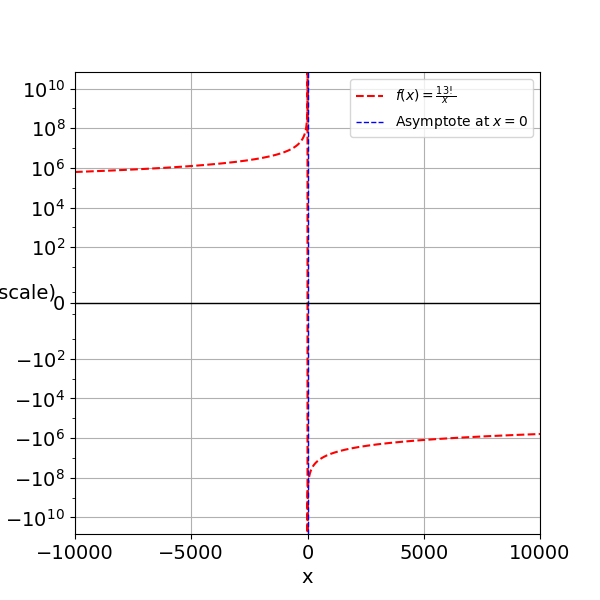
\includegraphics[width=0.8\textwidth]{Figure_1-assignment.png} 
    \caption{Graph showing the function \( f(x) = \frac{13!}{x} \) with asymptote at \( x = 0 \)}
    \label{fig:graph}
\end{figure}
multiset S = \{13, 13, NaN\}
\section*{Element 4 of multiset S}
Value is taken from task 3 and T3 = 0.
\\Therefore, multiset S = \{13, 13, NaN, 0\}

\section*{Propositional logic}
\vspace{.7cm}\[(13)(q \oplus p) \oplus r \leftrightarrow (\neg q \rightarrow \neg r)\] 

\vspace{.7cm}Where multiset S = \{13, 13, NaN, 0\}

\subsection*{ \[p = S \cap \{a, 0\} \equiv \{a\}\]}
p is false since the set of intersection is equal to \{a, 0\} and is not equivalent to \{a\}.

\subsection*{\[q = \{-\infty\} \subset S\]}
q is false, as negative infinity is not a subset of S.

\subsection*{\[r = S \cup \{0\} \subset S \]}
r is false as the multiset S U \{0\} is  \{13, 13, NaN, 0, 0\} and is not a subset of S.
\end{document}